Ogni tipo di modello di machine learning supervisionato può riscontrare, quando si trova ad operare
in contesti reali, un drift nelle distribuzioni dei dati osservati rispetto alla distribuzione
osservata durante la fase di addestramento. In particolare, uno dei tipi di modello più diffuso per il riconoscimento
delle immagini è quello che prende il nome di \textbf{rete neurale convolutiva} (Convolutional neural network, CNN).
In questo capitolo, introdurremo il funzionamento delle CNN e descriveremo l'architettura
utilizzata per questo progetto, le \textbf{reti neurali residuali}.
\section{Reti neurali convolutive}
Le \textbf{reti neurali convolutive} furono per la prima volta introdotte nella loro
forma moderna nel 1989 da Le Cun et al \cite{lecun_handwritten_1989}, i quali svilupparono LeNet-5, una
rete convolutiva in grado di classificare le cifre scritte a mano su dei fogli.
La struttura particolare di questo tipo di reti le rende particolarmente efficaci nell'ambito
del riconoscimento di immagini, poiché esse sono capaci di sfruttare le \textbf{caratteristiche spaziali dell'input}, come
per esempio la correlazione spaziale tra pixel vicini. Questa caratteristica permette inoltre di \textbf{ridurre il numero di pesi necessari da imparare},
rendendo quindi la rete più efficiente.
La figura \ref{fig:cnn_example} mostra l'architettura di LeNet-5 come esempio di rete neurale convolutiva.
Oltre ai layer di input e di output, le reti neurali convolutive sono formate principalmente da tre tipi di strati \cite{oshea_introduction_2015}:
\begin{itemize}
    \item Strati convolutivi
    \item Strati di pooling (o di subsampling)
    \item Strati completamente connessi
\end{itemize}
\begin{figure}
    \centering
    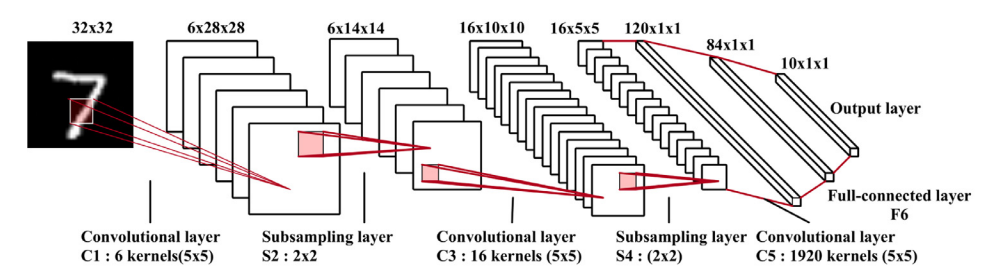
\includegraphics[width = \textwidth]{images/le-net.png}
    \caption{Architettura di LeNet-5. Da \cite{gu_recent_2018}}
    \label{fig:cnn_example}
\end{figure}
\subsubsection{Strato di input}
Come nelle reti neurali tradizionali, lo strato di input di una rete neurale convolutiva conterrà i valori delle istanze
che verranno passate alla rete. In particolare per le immagini, essi sono i \textbf{valori numerici dei suoi pixel}. Possiamo
quindi vedere un'immagine come una matrice di dimensioni $W \times H \times C$, con $W$ la larghezza dell'immagine, $H$ l'altezza dell'immagine
e $C$ il numero di \textbf{canali colore} (per esempio, $C =3$ se l'immagine ha canali colore RGB).
\subsubsection{Strati convolutivi}
Come abbiamo già detto sopra, le reti neurali convolutive sono in grado di sfruttare la struttura spaziale dell'input. Questo avviene nei \textbf{layer convolutivi}, il cui scopo è quello di imparare delle \textbf{rappresentazioni delle feature dell'input} \cite{gu_recent_2018}, cioè una rappresentazione delle caratteristiche presenti all'interno dell'input. Nel contesto delle immagini, esse possono essere, ad esempio, bordi, angoli, texture e forme.
L'apprendimento e l'estrazione di tali caratteristiche vengono effettuati avvalendosi di diversi \textbf{kernel convolutivi} (o filtri convolutivi), i quali vengono appresi dalla rete e utilizzati per effettuare una \textbf{convoluzione} sull'immagine. Più precisamente, il kernel viene fatto scorrere sull'input, considerando a ogni posizione una piccola regione locale di esso. Tale regione, rispetto al neurone che ne riceve le informazioni, viene definita \textbf{receptive field}. Viene quindi effettuato il prodotto scalare tra i valori presenti in questa regione e i pesi del kernel, ottenendo il valore di ingresso del neurone, il quale applicherà ad esso una funzione di attivazione non lineare per ottenere il suo valore di output, cioè la sua \textbf{attivazione}. Ripetendo questa operazione nelle diverse posizioni spaziali dell'input si ottiene una \textbf{feature map}, nella quale ogni valore corrisponde all'attivazione di un neurone in corrispondenza di una specifica regione dell'input. Ogni layer convolutivo si avvale di più kernel, i quali produrranno una feature map diversa ciascuno. Questo meccanismo ha diversi vantaggi:
\begin{itemize}
    \item Lo stesso kernel viene \textbf{condiviso tra tutte le posizioni spaziali dell'input}: in questo modo, lo stesso insieme di pesi viene utilizzato per rilevare una determinata caratteristica indipendentemente dalla sua posizione nell'immagine. Ciò inoltre diminuisce la complessità del modello, facilitandone l'addestramento.
    \item L'utilizzo di kernel differenti permette di ottenere diverse feature map, ciascuna delle quali può rappresentare una diversa caratteristica appresa dall'input
\end{itemize}
La figura \ref{fig:feature_maps} mostra un esempio di estrazione di feature maps in una CNN.
\begin{figure}
    \centering
    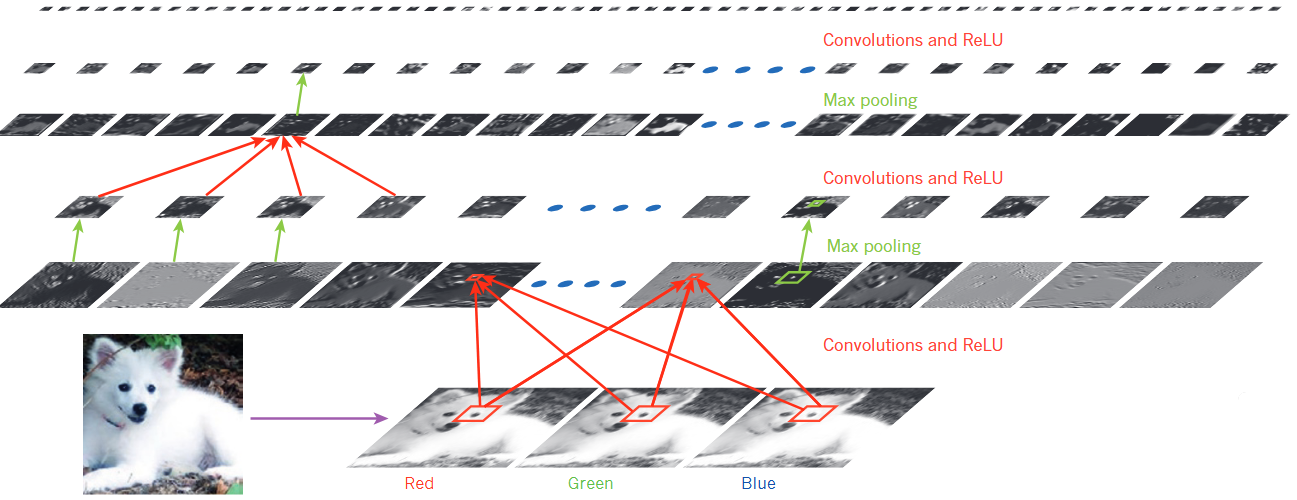
\includegraphics[width = \textwidth]{images/feature maps.png}
    \caption{Esempio di estrazione di feature map da un'immagine. Da \cite{lecun_deep_2015}}
    \label{fig:feature_maps}
\end{figure}
Infine, il kernel viene spostato sull'immagine di una quantità chiamata \textbf{stride}, che rappresenta il numero di pixel di cui il kernel viene traslato a ogni operazione di convoluzione. Di conseguenza, aumentando lo stride diminuisce il numero di posizioni nelle quali il kernel viene applicato e, in generale, si ottiene una \textbf{feature map} di dimensioni spaziali inferiori. Se i kernel della rete sono troppo grandi rispetto alle dimensioni dell'input, si può inoltre introdurre dello \textbf{zero padding} ai suoi bordi.
\subsubsection{Strati di pooling}
Lo scopo degli strati di pooling è quello di \textbf{ridurre le dimensioni spaziali delle feature map ottenute dai layer convolutivi} e, di conseguenza, ridurre la complessità computazionale del modello \cite{oshea_introduction_2015}. Anche questi layer si avvalgono di kernel per operare su piccole regioni spaziali dell'input. Tuttavia, a differenza degli strati convolutivi, questi kernel non possiedono parametri apprendibili e applicano generalmente una delle seguenti operazioni:
\begin{itemize}
    \item \textbf{Max-pooling}: viene selezionato il valore massimo tra quelli contenuti nella regione considerata.
    \item \textbf{Average-pooling}: viene calcolata la media dei valori contenuti nella regione considerata.
\end{itemize}
L'output di un layer di pooling sarà quindi una nuova \textbf{feature map} con dimensioni spaziali ridotte rispetto a quella in ingresso.  I layer di pooling sono generalmente posti tra due layer convolutivi e operano indipendentemente su ciascuna feature map. Combinando diversi layer convolutivi e di pooling, la rete può progressivamente estrarre caratteristiche sempre più complesse e di alto livello \cite{gu_recent_2018}.
\subsubsection{Strati completamente connessi}
% TODO: ricontrollare
Come in una rete neurale tradizionale, gli strati completamente connessi si occupano di \textbf{combinare le informazioni provenienti dallo strato precedente}, collegando ciascun neurone a tutti i neuroni dello strato precedente. In questo modo, le caratteristiche estratte dai layer convolutivi e vengono integrate per ottenere una rappresentazione globale dell'input \cite{gu_recent_2018}, che può essere successivamente utilizzata per effettuare la classificazione.
\subsubsection{Strato di ouput}
L'ultimo strato di una rete neurale convolutiva è lo strato di output, il quale si occupa di restituire il risultato della classificazione. Spesso, questo strato è rappresentato dall'operatore \textbf{softmax} oppure da una \textbf{SVM} \cite{gu_recent_2018}.
\section{Reti neurali residuali}
Le \textbf{reti neurali residuali} sono un'architettura per reti neurali profonde, proposto per la prima volta nel 2016 da He et al. \cite{he_deep_2016} e progettata per affrontare il problema della \textbf{degradazione}. Tale fenomeno si manifesta quando l'aumento della profondità della rete, ovvero del numero di layer, porta inizialmente a una saturazione dell'accuratezza e successivamente a un suo rapido decremento. Questo problema, inoltre, non è causato dall'overfitting, quindi aggiungere più layer alla rete porta ad un errore maggiore durante l'addestramento.  Per combattere questo fenomeno, le reti residuali adottano le seguenti soluzioni:
\begin{itemize}
    \item \textbf{Apprendimento residuale}: Consideriamo un insieme di layer di una rete neurale e supponiamo di voler fare in modo che essi apprendano un determinato mapping $\mathcal{H}(\boldsymbol{x})$, dove $\boldsymbol{x}$ rappresenta l'input fornito al primo dei layer considerati. Anziché apprendere direttamente il mapping desiderato, facciamo apprendere ai layer il \textbf{mapping residuale} $\mathcal{F}(\boldsymbol{x})$, definito come:
    $$\mathcal{F}(\boldsymbol{x}) \coloneqq \mathcal{H}(\boldsymbol{x}) - \boldsymbol{x}$$
    Di conseguenza, il mapping originale diventa:
    $$\mathcal{H}(\boldsymbol{x}) = \mathcal{F}(\boldsymbol{x}) + \boldsymbol{x}$$
    Questa riformulazione è giustificata dalla natura controintuitiva del problema della degradazione: la manifestazione di questo problema potrebbe indicare che i solver di ottimizzazione faticano ad approssimare l'identità componendo più layer non lineari. Riformulando il mapping in questo modo, l'ottimizzazione diventa più semplice: se il mapping ottimale è vicino all'identità, è sufficiente che i pesi dei layer tendano a zero.
    \item \textbf{Identity shortcut connections}: Il mapping $\mathcal{F}(\boldsymbol{x}) + \boldsymbol{x}$ può essere realizzato da una rete dotata di "shortcut connections", ovvero connessioni che saltano uno o più layer della rete. Nel caso delle reti residuali, queste connessioni collegano semplicemente l'input di un gruppo di layer alla sua uscita, sommando l'identità $\boldsymbol{x}$ all'output dei layer.
\end{itemize}
\begin{figure}
    \centering
    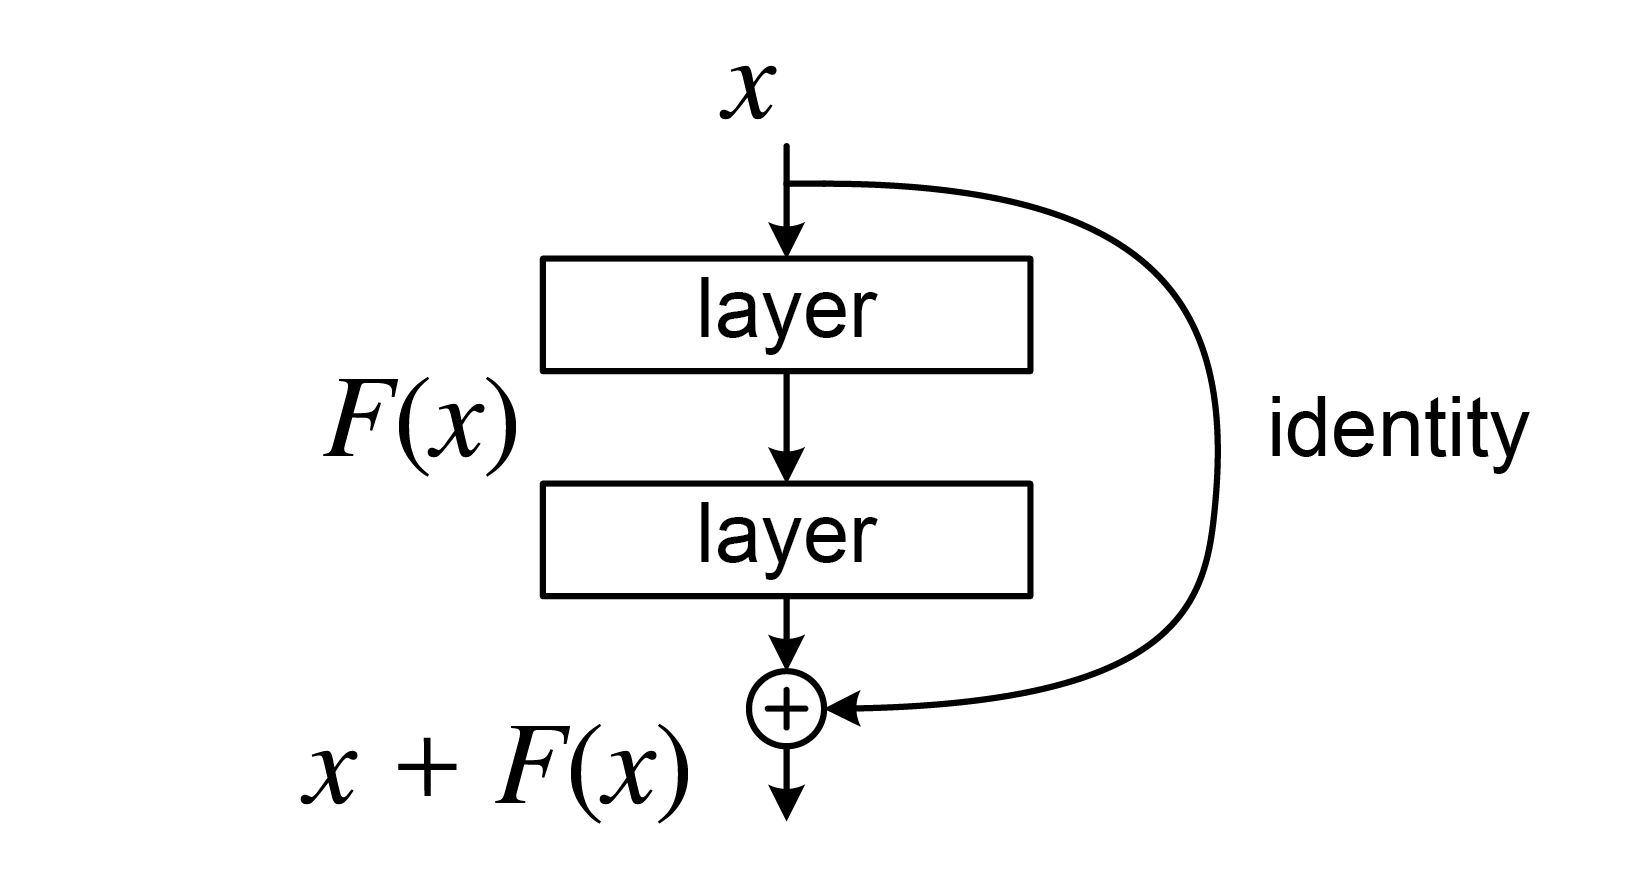
\includegraphics[width = 0.55\textwidth]{images/resnet.png}
    \caption{Esempio di blocco residuale. Da \cite{he_deep_2016}}
    \label{fig:residual_block}
\end{figure}
La figura \ref{fig:residual_block} mostra un esempio di blocco residuale. Queste soluzioni portano ad ottenere reti più facili da ottimizzare rispetto alle reti neurali profonde tradizionali e in grado di trarre maggiore beneficio, in termini di accuratezza, dall'aumento della profondità.
\subsection{ResNet50}
I modelli sviluppati da He et al. in \cite{he_deep_2016} sono stati addestrati e valutati su ImageNet-1k. Uno di questi modelli è ResNet50, il quale viene utilizzato come modello per questo progetto.  
Le versioni di rete residuale più profonde, tra cui ResNet50, adottano un blocco residuo differente rispetto a quello base a due layer utilizzato nelle versioni meno profonde: per contenere i tempi di addestramento, ogni funzione residuale $\mathcal{F}$ viene realizzata tramite tre layer convolutivi di dimensioni rispettivamente $1 \times 1$, $3 \times 3$ e $1 \times 1$, detti \textbf{layer di bottleneck}. Il primo e l'ultimo layer si occupano rispettivamente di ridurre e successivamente ricostruire le dimensioni dell'input, mentre il layer $3 \times 3$ centrale opera come un "collo di bottiglia" (\textit{bottleneck}), con dimensioni di input e output ridotte rispetto al resto del blocco. Questo cambiamento non comporta nessun aumento significativo della complessità computazionale, la quale resta simile rispetto all'implementazione a due blocchi. Un esempio di blocco "bottleneck" è mostrato in figura \ref{fig:bottleneck}
\begin{figure}
    \centering
    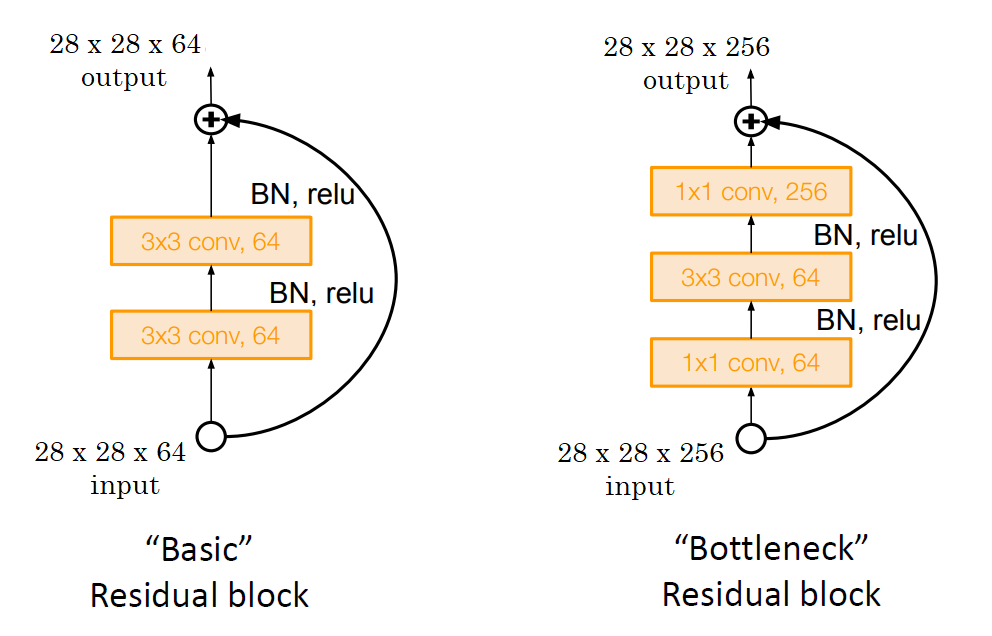
\includegraphics[width = 0.65\textwidth]{images/bottleneck.PNG}
    \caption{Confronto tra un blocco residuale e un blocco "bottleneck". Da \cite{he_deep_2016}}
    \label{fig:bottleneck}
\end{figure}